\documentclass[10pt]{beamer}

% ------------------------------------------------------------------------
% Carga del preámbulo personalizado
% (Asegúrate de contar con preamble.tex en la misma carpeta,
%  donde defines temas, colores, macros como \myfront, etc.)
% ------------------------------------------------------------------------
\usetheme[progressbar=frametitle]{metropolis}
\usepackage{appendixnumberbeamer}
\usepackage{fancyvrb}
\usepackage{booktabs}
\usepackage[scale=2]{ccicons}
\usepackage{pgfplots}
\usepgfplotslibrary{dateplot}
\usepackage{type1cm}
\usepackage{lettrine}
\usepackage{ragged2e}
\usepackage{xspace}
\newcommand{\themename}{\textbf{\textsc{metropolis}}\xspace}
\usepackage{graphicx} % Allows including images
\usepackage{booktabs} % Allows the use of \toprule, \midrule and \bottomrule in tables
\usepackage[utf8]{inputenc} %solucion del problema de los acentos.
\usepackage{xcolor}
\definecolor{LightGray}{gray}{0.9}

\usepackage{minted}
\usemintedstyle{tango}
\newcommand{\mypyfile}[1]{\inputminted[linenos=true, fontsize=\footnotesize, frame=lines, framesep=5\fboxrule,framerule=1pt]{python}{#1}}

\setminted[python]{breaklines,frame=lines,framesep=2mm,baselinestretch=1.2,bgcolor=LightGray,linenos, fontsize=\footnotesize} % obeytabs=true, tabsize=2, showtabs=true}

%%%%%%%%%%%%%%%%%%%%%%%%%%%%%%%%%%%%%%%%%%%%%%%%%%%%%%%%%%%%%%%%%%%%%%%%%%%%%%%%%%%%%%
\setbeamercolor{progress bar}{fg=blue!50!black,bg=white!50!black}
\setbeamercolor{title separator}{fg=red!50!black,bg=white!50!black}
\setbeamercolor{frametitle}{fg=white!80!black,bg=red!50!black}
\title[PCFI161]{Programaci\'on para F\'isica y Astronom\'ia}
\subtitle{Departamento de Física.}

\newcommand{\myfront}{
\author[PCFI161]{Corodinadora: C Loyola \\ Profesoras/es C Loyola / C Femenías / Y Navarrete / C Ruiz}
\institute[UNAB]{Universidad Andrés Bello}
\date{Primer Semestre 2025}
}

\titlegraphic{%
  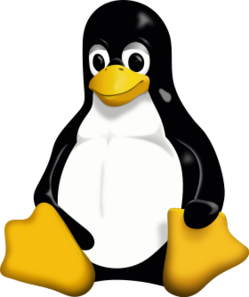
\includegraphics[width=.08\textwidth]{logo-tux.png}\hfill
  
\includegraphics[width=.3\textwidth]{logo-unab.png}\hfill
  
\includegraphics[width=.08\textwidth]{logo-python.png}
}

\makeatletter
\setbeamertemplate{title page}{
  \begin{minipage}[b][\paperheight]{\textwidth}
    \vfill%
    \ifx\inserttitle\@empty\else\usebeamertemplate*{title}\fi
    \ifx\insertsubtitle\@empty\else\usebeamertemplate*{subtitle}\fi
    \usebeamertemplate*{title separator}
    \ifx\beamer@shortauthor\@empty\else\usebeamertemplate*{author}\fi
    \ifx\insertdate\@empty\else\usebeamertemplate*{date}\fi
    \ifx\insertinstitute\@empty\else\usebeamertemplate*{institute}\fi
    \vfill
    \ifx\inserttitlegraphic\@empty\else\inserttitlegraphic\fi
    \vspace*{1cm}
  \end{minipage}
}
\makeatother


\makeatletter
\setlength{\metropolis@titleseparator@linewidth}{2pt}
\setlength{\metropolis@progressonsectionpage@linewidth}{2pt}
\setlength{\metropolis@progressinheadfoot@linewidth}{2pt}
\makeatother


\begin{document}

% ------------------------------------------------------------------------
% Portada personalizada. Por ejemplo, usando \myfront si lo tienes en el preámbulo.
% ------------------------------------------------------------------------
\myfront{}

% ------------------------------------------------------------------------
% SLIDE 1: Título de la segunda sesión
% ------------------------------------------------------------------------
\begin{frame}
  \titlepage
  % Puedes ajustar el título/subtítulo para esta sesión específica
  % por ejemplo: \title{Sesión 2 - Semana 1: Ejercicios Iniciales en Colab}
\end{frame}

% ------------------------------------------------------------------------
% SLIDE 2: Índice / Tabla de contenidos
% ------------------------------------------------------------------------
\begin{frame}
  \frametitle{Resumen - Sesión 2 (Semana 1)}
  \tableofcontents
\end{frame}

% ------------------------------------------------------------------------
% Configuración de bloques (en caso de usar metrópolis u otro tema)
% ------------------------------------------------------------------------
\metroset{block=fill}

% ----------------------------------------------------------------------------------------
% SECCIÓN 1: Recapitulación de la Sesión 1
% ----------------------------------------------------------------------------------------
\section{Introducción y Repaso}

% ------------------------------------------------------------------------
% Slide 3: Repaso Rápido
% ------------------------------------------------------------------------
\begin{frame}{Repaso de la Sesión Anterior}
  \begin{itemize}
    \item Contexto general del curso y relevancia de la programación en Física/Astronomía.
    \item Familiarización inicial con Google Colab:
      \begin{itemize}
        \item Creación de notebooks.
        \item Ejecución de código básico.
      \end{itemize}
    \item Introducción a los tipos de datos y operaciones simples (asignaciones, suma, resta, etc.).
    \item Primeros ejemplos de entrada y salida (\texttt{input()}, \texttt{print()}).
  \end{itemize}
\end{frame}

% ------------------------------------------------------------------------
% Slide 4: Objetivos de Esta Sesión
% ------------------------------------------------------------------------
\begin{frame}{Objetivos de la Sesión 2}
  \begin{itemize}
    \item \textbf{Practicar} asignaciones simples y operaciones aritméticas en Colab.
    \item \textbf{Explorar} más ejemplos de entrada/salida y la ejecución inmediata de código.
    \item \textbf{Fomentar} la colaboración e intercambio de estrategias entre estudiantes.
    \item \textbf{Resolver} ejercicios que integren los conceptos vistos en la sesión anterior.
  \end{itemize}
\end{frame}

% ----------------------------------------------------------------------------------------
% SECCIÓN 2: Warm-up - Preparación para la Práctica
% ----------------------------------------------------------------------------------------
\section{Preparación para la Práctica}

% ------------------------------------------------------------------------
% Slide 5: Recordatorio de Conceptos Clave
% ------------------------------------------------------------------------
\begin{frame}{Recordatorio: Conceptos Clave de la Sesión 1}
  \begin{itemize}
    \item \textbf{Variables y Asignación}: \texttt{nombre = valor}
    \item \textbf{Tipos de datos}: \texttt{int}, \texttt{float}, \texttt{str}
    \item \textbf{Entrada}: \texttt{input()} siempre devuelve string
    \item \textbf{Conversión}: \texttt{float()}, \texttt{int()}
    \item \textbf{Salida}: \texttt{print()} y f-strings
  \end{itemize}
  
  \begin{block}{Patrón básico de un programa}
    \texttt{entrada → procesamiento → salida}
  \end{block}
\end{frame}

% ------------------------------------------------------------------------
% Slide 6: Demostración Rápida en Vivo
% ------------------------------------------------------------------------
\begin{frame}[fragile]{Demostración en Vivo: Recordando lo Básico}
\begin{minted}{python}
# Ejemplo simple para refrescar
nombre = input("¿Cómo te llamas? ")
edad = int(input("¿Cuántos años tienes? "))

print(f"Hola {nombre}, tienes {edad} años")

# Operación matemática simple
area = 3.14 * 5**2
print(f"Área de círculo radio 5: {area}")
\end{minted}

\textbf{Ejecutemos esto juntos} para recordar la mecánica básica.
\end{frame}

% ----------------------------------------------------------------------------------------
% SECCIÓN 3: Ejercicios Guiados (Progresión Gradual)
% ----------------------------------------------------------------------------------------
\section{Ejercicios Guiados}

% ------------------------------------------------------------------------
% Slide 7: Ejercicio 1 - Área y Perímetro de Rectángulo
% ------------------------------------------------------------------------
\begin{frame}{Ejercicio 1: \hfill \textcolor{red}{$\clubsuit$} \\ Área y Perímetro de un Rectángulo}
  \begin{block}{Enunciado}
    \begin{itemize}
      \item Solicita al usuario el largo y ancho de un rectángulo (en metros).
      \item Calcula el área (\(A = largo \times ancho\)) y el perímetro (\(P = 2(largo + ancho)\)).
      \item Muestra ambos resultados con unidades apropiadas.
    \end{itemize}
  \end{block}
  
  \textbf{Trabajemos este ejercicio JUNTOS paso a paso:}
  \begin{enumerate}
    \item Identificar las entradas necesarias
    \item Escribir las fórmulas matemáticas
    \item Implementar en Python
    \item Probar con valores específicos
  \end{enumerate}
\end{frame}

% ------------------------------------------------------------------------
% Slide 8: Solución Ejercicio 1 (Paso a Paso)
% ------------------------------------------------------------------------
\begin{frame}[fragile]{Solución Ejercicio 1: \hfill \textcolor{green}{$\checkmark$} \\ Paso a Paso}
\begin{minted}{python}
# Paso 1: Obtener datos del usuario
largo = float(input("Largo del rectángulo (m): "))
ancho = float(input("Ancho del rectángulo (m): "))

# Paso 2: Calcular usando las fórmulas
area = largo * ancho
perimetro = 2 * (largo + ancho)

# Paso 3: Mostrar resultados con formato claro
print(f"Área: {area} m²")
print(f"Perímetro: {perimetro} m")
\end{minted}

\textbf{Probemos con}: largo = 5, ancho = 3
\textbf{Resultado esperado}: Área = 15 m², Perímetro = 16 m
\end{frame}


% ----------------------------------------------------------------------------------------
% SECCIÓN 4: Práctica Individual/Grupal
% ----------------------------------------------------------------------------------------
\section{Práctica Colaborativa}

% ------------------------------------------------------------------------
% Slide : Grupos de Trabajo
% ------------------------------------------------------------------------
\begin{frame}{Trabajo en Grupos}
  \begin{itemize}
    \item Dividir la clase en \textbf{equipos de 2-3 integrantes}.
    \item Cada integrante del equipo crea su propio notebook en Colab.
    \item Se recomienda comentar el código para anotar:
      \begin{itemize}
        \item Qué hace cada línea.
        \item Si surge algún error, cómo se corrigió.
      \end{itemize}
    \item Comparar sus resultados y conclusiones.
    \item Importante a cada integrante le funcione el código en su notebook.
  \end{itemize}
\end{frame}

% ------------------------------------------------------------------------
% Slide : Puesta en Común
% ------------------------------------------------------------------------
\begin{frame}{Puesta en Común de Dudas y Experiencias}
  \begin{itemize}
    \item Cada equipo expondrá brevemente:
      \begin{itemize}
        \item ¿Qué ejercicio les costó más y por qué?
        \item ¿Cómo resolvieron los problemas encontrados?
        \item ¿Algún atajo o truco que consideren útil?
      \end{itemize}
    \item Se fomenta la retroalimentación colectiva.
    \item \textbf{Tip:} Documentar buenas prácticas que surjan de la discusión.
  \end{itemize}
\end{frame}


% ------------------------------------------------------------------------
% Slide 7: Ejercicio 2 - Calculadora de Velocidad
% ------------------------------------------------------------------------
\begin{frame}{Ejercicio 2: \hfill \textcolor{red}{$\clubsuit$}\\ Calculadora de Velocidad}
  \begin{block}{Enunciado}
    \begin{itemize}
      \item Pide al usuario la distancia recorrida (en metros) y el tiempo empleado (en segundos).
      \item Calcula la velocidad usando la fórmula \(v = \frac{d}{t}\).
      \item Muestra el resultado en m/s y también convertido a km/h.
    \end{itemize}
  \end{block}
  \textbf{Conversión:} Para pasar de m/s a km/h, multiplicar por 3.6.
  \\
  \textbf{Física:} Esta es una de las ecuaciones cinemáticas fundamentales.
\end{frame}

% ------------------------------------------------------------------------
% Slide 8: Ejercicio 3 - Suma de Dos Variables
% ------------------------------------------------------------------------
\begin{frame}{Ejercicio 3: \hfill \textcolor{red}{$\clubsuit$} \\ Suma de Dos Variables}
  \begin{block}{Enunciado}
    \begin{itemize}
      \item Pide al usuario dos números (pueden ser enteros o decimales).
      \item Asigna cada número a una variable distinta (\texttt{a, b}).
      \item Realiza la suma y muestra el resultado.
    \end{itemize}
  \end{block}
  \textbf{Extensión:} Imprime también la resta, el producto y el cociente.
\end{frame}

% ------------------------------------------------------------------------
% Slide 9: Ejercicio 4 - Promedio de Tres Notas
% ------------------------------------------------------------------------
\begin{frame}{Ejercicio 4: \hfill \textcolor{red}{$\clubsuit$} \\ Promedio de Tres Notas }
  \begin{block}{Enunciado}
    \begin{itemize}
      \item Solicita tres notas (numeros en \([1.0 - 7.0]\) típicamente).
      \item Calcula el promedio aritmético.
      \item Muestra el resultado con un mensaje apropiado.
    \end{itemize}
  \end{block}
  \textbf{Discusión:}
  \begin{itemize}
    \item ¿Qué pasa si ingresan valores fuera del rango?
    \item El tipo de dato a usar: \texttt{float}.
  \end{itemize}
\end{frame}

% ------------------------------------------------------------------------
% Slide 10: Ejercicio 5 - Conversión de Temperatura
% ------------------------------------------------------------------------
\begin{frame}{Ejercicio 5: \hfill \textcolor{red}{$\clubsuit$} \\ Conversión de Temperatura}
  \begin{block}{Enunciado}
    \begin{itemize}
      \item Pide una temperatura en grados Celsius.
      \item Convierte a Fahrenheit: \(F = \frac{9}{5}C + 32\)
      \item Convierte a Kelvin: \(K = C + 273.15\)
      \item Muestra los tres valores con sus unidades.
    \end{itemize}
  \end{block}
  
  \textbf{Prueben con}: 0°C, 100°C, -40°C
  \\
  \textbf{Física relevante}: Estas conversiones son fundamentales en física y astronomía.
\end{frame}



% ------------------------------------------------------------------------
% Slide 12: Ejemplo de Solución (Calculadora de Velocidad)
% ------------------------------------------------------------------------
\begin{frame}[fragile]{Solución 2 de Referencia: \hfill \textcolor{green}{$\checkmark$} \\ Calculadora de Velocidad}
\begin{minted}{python}
distancia = float(input("Distancia recorrida (m): "))
tiempo = float(input("Tiempo empleado (s): "))

velocidad_ms = distancia / tiempo
velocidad_kmh = velocidad_ms * 3.6

print(f'Velocidad: {velocidad_ms} m/s')
print(f'Velocidad: {velocidad_kmh} km/h')
\end{minted}
\textbf{Discusión:} ¿Qué ocurre si tiempo = 0? (División por cero)
\end{frame}

% ------------------------------------------------------------------------
% Slide 13: Ejemplo de Solución (Suma de Dos Variables)
% ------------------------------------------------------------------------
\begin{frame}[fragile]{Solución 3 de Referencia: \hfill \textcolor{green}{$\checkmark$} \\Suma de Dos Variables}
\begin{minted}{python}
a_str = input("Ingresa el primer número: ")
b_str = input("Ingresa el segundo número: ")

a = float(a_str)
b = float(b_str)

suma = a + b
resta = a - b
producto = a * b
cociente = a / b  # Cuidar la división por cero

print(f'Suma = {suma}')
print(f'Resta = {resta}')
print(f'Producto = {producto}')
print(f'Cociente = {cociente}')
\end{minted}
\end{frame}

% ------------------------------------------------------------------------
% Slide 14: Ejemplo de Solución (Promedio de Tres Notas)
% ------------------------------------------------------------------------
\begin{frame}[fragile]{Solución 4 de Referencia: \hfill \textcolor{green}{$\checkmark$} \\Promedio de Tres Notas}
\begin{minted}{python}
n1 = float(input("Nota 1: "))
n2 = float(input("Nota 2: "))
n3 = float(input("Nota 3: "))

promedio = (n1 + n2 + n3) / 3
print(f'El promedio de las tres notas es: {promedio}')
\end{minted}
\textbf{Discusión:} Manejo de rangos y validaciones (opcional).
\end{frame}

% ------------------------------------------------------------------------
% Slide 13: Soluciones de Referencia - Ejercicio 5
% ------------------------------------------------------------------------
\begin{frame}[fragile]{Solución 5 de Referencia: \hfill \textcolor{green}{$\checkmark$} \\ Conversión de Temperatura}
\begin{minted}{python}
celsius = float(input("Temperatura en °C: "))

fahrenheit = (9/5) * celsius + 32
kelvin = celsius + 273.15

print(f"Temperatura en °C: {celsius}")
print(f"Temperatura en °F: {fahrenheit}")
print(f"Temperatura en K: {kelvin}")
\end{minted}

\textbf{Verificación}:
\begin{itemize}
  \item 0°C = 32°F = 273.15K
  \item 100°C = 212°F = 373.15K
  \item -40°C = -40°F = 233.15K
\end{itemize}
\end{frame}

\section{Errores Comunes y Mejores Prácticas}

% ------------------------------------------------------------------------
% Slide 15: Pequeña Discusión sobre Errores
% ------------------------------------------------------------------------
\begin{frame}{Errores Comunes en Esta Sesión}
  \begin{block}{Errores frecuentes}
    \begin{itemize}
      \item \textbf{ValueError}: Intentar convertir texto no numérico a \texttt{float()}
      \item \textbf{NameError}: Escribir mal el nombre de una variable
      \item \textbf{ZeroDivisionError}: División por cero
      \item \textbf{SyntaxError}: Olvidar comillas, paréntesis, etc.
    \end{itemize}
  \end{block}
  
  \begin{alertblock}{Consejo}
    Los errores son \textbf{oportunidades de aprendizaje}. Python te dice exactamente dónde está el problema y qué tipo de error es.
  \end{alertblock}
\end{frame}

% ------------------------------------------------------------------------
% Slide 16: Buenas Prácticas Observadas
% ------------------------------------------------------------------------
\begin{frame}{Buenas Prácticas que Esperamos Ver}
  \begin{itemize}
    \item \textbf{Nombres descriptivos}: \texttt{celsius} en lugar de \texttt{c}
    \item \textbf{Comentarios útiles}: Explicar fórmulas complejas
    \item \textbf{Incluir unidades}: en mensajes de entrada y salida
    \item \textbf{Probar con casos extremos}: valores grandes, pequeños, cero
    \item \textbf{Formato claro}: usar f-strings para salidas legibles
  \end{itemize}
  
  \begin{block}{Ejemplo de buen estilo}
    \texttt{temperatura\_celsius = float(input("Ingrese temperatura en °C: "))}
  \end{block}
\end{frame}


% ----------------------------------------------------------------------------------------
% SECCIÓN 5: Actividad Adicional y Retroalimentación
% ----------------------------------------------------------------------------------------
\section{Actividades Extra}

% ------------------------------------------------------------------------
% Slide 16: Actividad Extra - Escalas Físicas
% ------------------------------------------------------------------------
\begin{frame}{Actividad Extra 1: Escalas Físicas}
  El objetivo de esta actividad es de práctica en casa, la idea es que pueda prepararse para la Tarea en clase de la próxima semana que se realizará en la sesión 2.
  \begin{block}{Enunciado}
    \begin{itemize}
      \item Pide la temperatura en \(^\circ C\) y conviértela a \(^\circ F\) y K.
      \item Pide la masa en kg y conviértela a libras.
      \item Muestra un pequeño resumen en pantalla con los resultados.
    \end{itemize}
  \end{block}
  \textbf{Objetivo:} Reforzar uso de variables, operaciones aritméticas y \texttt{print}.
\end{frame}

% ------------------------------------------------------------------------
% Slide 17: Mini-Reto - Operaciones con Complejos
% ------------------------------------------------------------------------
\begin{frame}{Actividad Extra 2: \\ Números Complejos (Opcional)}
  \begin{itemize}
    \item Python maneja complejos con la letra \texttt{j} (\emph{ej}: \texttt{3+2j}).
    \item Investiga cómo sumar, restar y multiplicar números complejos.
    \item \textbf{Ejemplo}:
      \[
        z1 = 3 + 4j, \quad z2 = 2 - 1j
      \]
      \[
        z3 = z1 * z2
      \]
      \(\dots\) Imprime \(\operatorname{Re}(z3)\) y \(\operatorname{Im}(z3)\).
    \item \textbf{Tip}: Usa \texttt{z.real} y \texttt{z.imag} para acceder a sus partes real e imaginaria.
  \end{itemize}
\end{frame}

% ------------------------------------------------------------------------
% Slide 18: Momento de Discusión
% ------------------------------------------------------------------------
\begin{frame}{Discusión Grupales y Dudas}
  \begin{itemize}
    \item ¿Qué soluciones o trucos surgieron durante la actividad extra?
    \item ¿Se presentaron nuevas dudas o errores inesperados?
    \item ¿Qué parte de Python se está volviendo más clara y qué sigue siendo confuso?
  \end{itemize}
  \begin{block}{IMPORTANTE!!!}
    Los resultados de su trabajo en clases deben ser entregados mediante la plataforma CANVAS.
  \end{block}
\end{frame}

% ------------------------------------------------------------------------
% Slide 19: Retroalimentación y Comentarios
% ------------------------------------------------------------------------
\begin{frame}{Retroalimentación}
  \begin{itemize}
    \item Comparte tu experiencia de aprendizaje con tus compañeros.
    \item \textbf{Ventajas} de Colab: ejecución inmediata, trabajo colaborativo, fácil despliegue de resultados.
    \item \textbf{Desafíos} detectados: conexión a internet, diferencia de versiones, etc.
  \end{itemize}
\end{frame}

% ----------------------------------------------------------------------------------------
% SECCIÓN 6: Conclusiones y Próximos Pasos
% ----------------------------------------------------------------------------------------
\section{Conclusiones}

% ------------------------------------------------------------------------
% Slide 20: Resumen de la Sesión 2
% ------------------------------------------------------------------------
\begin{frame}{Resumen de la Sesión 2}
  \begin{itemize}
    \item Reforzamos las operaciones básicas y la asignación de variables.
    \item Practicamos \textbf{entrada/salida} con varios ejemplos.
    \item Exploramos la \textit{ejecución inmediata} de celdas en Colab y la importancia del orden.
    \item Fomentamos la resolución colaborativa para intercambiar estrategias.
  \end{itemize}
\end{frame}

% ------------------------------------------------------------------------
% Slide 21: Enfoque para la Próxima Sesión
% ------------------------------------------------------------------------
\begin{frame}{Próximos Pasos}
  \begin{itemize}
    \item \textbf{Sesión 3 (Semana 2)}: Introducción a estructuras de control (\texttt{if}, \texttt{while}).
    \item \textbf{Explotaremos} ejemplos físicos básicos (análisis de condiciones, pequeños bucles, etc.).
    \item \textbf{Revisión previa}: Asegúrate de dominar los \textbf{tipos de datos} y la conversión de \texttt{input()} a \texttt{float}.
  \end{itemize}
\end{frame}

% ------------------------------------------------------------------------
% Slide 22: Referencias y Recursos
% ------------------------------------------------------------------------
\begin{frame}{Recursos Recomendados}
  \begin{itemize}
    \item \textbf{Para practicar Python:} \href{https://www.hackerrank.com/domains/python?filters\%5Bdifficulty\%5D\%5B\%5D=easy}{HackerRank - Python Practice}
    \item \textbf{Documentación Python:} \href{https://docs.python.org/3/}{docs.python.org/3}
    \item \textbf{Tutoriales en línea:} W3Schools, Real Python.
    \item \textbf{Comunidades:} Stack Overflow, Reddit \texttt{/r/learnpython}.
    \item \textbf{GitHub:} Busca \emph{“intro to python for physics”} para ejemplos.
  \end{itemize}
\end{frame}

% ------------------------------------------------------------------------
% Slide 23: Comentarios Finales
% ------------------------------------------------------------------------
\begin{frame}{Comentarios Finales}
  \begin{itemize}
    \item \textbf{Practicar} es fundamental: domina bien asignaciones y operaciones antes de pasar a estructuras más complejas.
    \item \textbf{Comparte} dudas en foros o con tus compañeros.
    \item \textbf{Recuerda}: Python es sensible a mayúsculas y espacios en la indentación (veremos más en bucles).
  \end{itemize}
\end{frame}

% ------------------------------------------------------------------------
% Slide 24: Invitación a Explorar
% ------------------------------------------------------------------------
\begin{frame}{Invitación a Explorar por tu Cuenta}
  \begin{itemize}
    \item Juega con \textbf{sentencias de asignación} para ver cómo cambiar valores.
    \item Crea \textbf{pequeños scripts} con 2-3 entradas distintas.
    \item Prueba \textbf{operaciones} con números \emph{muy grandes} y \emph{muy pequeños}.
    \item Observa cómo Python maneja la \textit{precisión} numérica.
  \end{itemize}
\end{frame}

% ------------------------------------------------------------------------
% Slide 25: Cierre de la Sesión
% ------------------------------------------------------------------------
\begin{frame}
  \huge{\centerline{¡Gracias y hasta la próxima sesión!}}
  \vspace{0.4cm}
  \normalsize
  \begin{itemize}
    \item Recuerda guardar tus notebooks en Drive.
    \item Si te sobró tiempo, continúa con los mini-retos.
    \item ¡Nos vemos en la Semana 2 con más Python!
  \end{itemize}
\end{frame}

\end{document}

